% Options for packages loaded elsewhere
\PassOptionsToPackage{unicode}{hyperref}
\PassOptionsToPackage{hyphens}{url}
%
\documentclass[
]{article}
\usepackage{amsmath,amssymb}
\usepackage{iftex}
\ifPDFTeX
  \usepackage[T1]{fontenc}
  \usepackage[utf8]{inputenc}
  \usepackage{textcomp} % provide euro and other symbols
\else % if luatex or xetex
  \usepackage{unicode-math} % this also loads fontspec
  \defaultfontfeatures{Scale=MatchLowercase}
  \defaultfontfeatures[\rmfamily]{Ligatures=TeX,Scale=1}
\fi
\usepackage{lmodern}
\ifPDFTeX\else
  % xetex/luatex font selection
\fi
% Use upquote if available, for straight quotes in verbatim environments
\IfFileExists{upquote.sty}{\usepackage{upquote}}{}
\IfFileExists{microtype.sty}{% use microtype if available
  \usepackage[]{microtype}
  \UseMicrotypeSet[protrusion]{basicmath} % disable protrusion for tt fonts
}{}
\makeatletter
\@ifundefined{KOMAClassName}{% if non-KOMA class
  \IfFileExists{parskip.sty}{%
    \usepackage{parskip}
  }{% else
    \setlength{\parindent}{0pt}
    \setlength{\parskip}{6pt plus 2pt minus 1pt}}
}{% if KOMA class
  \KOMAoptions{parskip=half}}
\makeatother
\usepackage{xcolor}
\usepackage[margin=1in]{geometry}
\usepackage{color}
\usepackage{fancyvrb}
\newcommand{\VerbBar}{|}
\newcommand{\VERB}{\Verb[commandchars=\\\{\}]}
\DefineVerbatimEnvironment{Highlighting}{Verbatim}{commandchars=\\\{\}}
% Add ',fontsize=\small' for more characters per line
\usepackage{framed}
\definecolor{shadecolor}{RGB}{248,248,248}
\newenvironment{Shaded}{\begin{snugshade}}{\end{snugshade}}
\newcommand{\AlertTok}[1]{\textcolor[rgb]{0.94,0.16,0.16}{#1}}
\newcommand{\AnnotationTok}[1]{\textcolor[rgb]{0.56,0.35,0.01}{\textbf{\textit{#1}}}}
\newcommand{\AttributeTok}[1]{\textcolor[rgb]{0.13,0.29,0.53}{#1}}
\newcommand{\BaseNTok}[1]{\textcolor[rgb]{0.00,0.00,0.81}{#1}}
\newcommand{\BuiltInTok}[1]{#1}
\newcommand{\CharTok}[1]{\textcolor[rgb]{0.31,0.60,0.02}{#1}}
\newcommand{\CommentTok}[1]{\textcolor[rgb]{0.56,0.35,0.01}{\textit{#1}}}
\newcommand{\CommentVarTok}[1]{\textcolor[rgb]{0.56,0.35,0.01}{\textbf{\textit{#1}}}}
\newcommand{\ConstantTok}[1]{\textcolor[rgb]{0.56,0.35,0.01}{#1}}
\newcommand{\ControlFlowTok}[1]{\textcolor[rgb]{0.13,0.29,0.53}{\textbf{#1}}}
\newcommand{\DataTypeTok}[1]{\textcolor[rgb]{0.13,0.29,0.53}{#1}}
\newcommand{\DecValTok}[1]{\textcolor[rgb]{0.00,0.00,0.81}{#1}}
\newcommand{\DocumentationTok}[1]{\textcolor[rgb]{0.56,0.35,0.01}{\textbf{\textit{#1}}}}
\newcommand{\ErrorTok}[1]{\textcolor[rgb]{0.64,0.00,0.00}{\textbf{#1}}}
\newcommand{\ExtensionTok}[1]{#1}
\newcommand{\FloatTok}[1]{\textcolor[rgb]{0.00,0.00,0.81}{#1}}
\newcommand{\FunctionTok}[1]{\textcolor[rgb]{0.13,0.29,0.53}{\textbf{#1}}}
\newcommand{\ImportTok}[1]{#1}
\newcommand{\InformationTok}[1]{\textcolor[rgb]{0.56,0.35,0.01}{\textbf{\textit{#1}}}}
\newcommand{\KeywordTok}[1]{\textcolor[rgb]{0.13,0.29,0.53}{\textbf{#1}}}
\newcommand{\NormalTok}[1]{#1}
\newcommand{\OperatorTok}[1]{\textcolor[rgb]{0.81,0.36,0.00}{\textbf{#1}}}
\newcommand{\OtherTok}[1]{\textcolor[rgb]{0.56,0.35,0.01}{#1}}
\newcommand{\PreprocessorTok}[1]{\textcolor[rgb]{0.56,0.35,0.01}{\textit{#1}}}
\newcommand{\RegionMarkerTok}[1]{#1}
\newcommand{\SpecialCharTok}[1]{\textcolor[rgb]{0.81,0.36,0.00}{\textbf{#1}}}
\newcommand{\SpecialStringTok}[1]{\textcolor[rgb]{0.31,0.60,0.02}{#1}}
\newcommand{\StringTok}[1]{\textcolor[rgb]{0.31,0.60,0.02}{#1}}
\newcommand{\VariableTok}[1]{\textcolor[rgb]{0.00,0.00,0.00}{#1}}
\newcommand{\VerbatimStringTok}[1]{\textcolor[rgb]{0.31,0.60,0.02}{#1}}
\newcommand{\WarningTok}[1]{\textcolor[rgb]{0.56,0.35,0.01}{\textbf{\textit{#1}}}}
\usepackage{graphicx}
\makeatletter
\def\maxwidth{\ifdim\Gin@nat@width>\linewidth\linewidth\else\Gin@nat@width\fi}
\def\maxheight{\ifdim\Gin@nat@height>\textheight\textheight\else\Gin@nat@height\fi}
\makeatother
% Scale images if necessary, so that they will not overflow the page
% margins by default, and it is still possible to overwrite the defaults
% using explicit options in \includegraphics[width, height, ...]{}
\setkeys{Gin}{width=\maxwidth,height=\maxheight,keepaspectratio}
% Set default figure placement to htbp
\makeatletter
\def\fps@figure{htbp}
\makeatother
\setlength{\emergencystretch}{3em} % prevent overfull lines
\providecommand{\tightlist}{%
  \setlength{\itemsep}{0pt}\setlength{\parskip}{0pt}}
\setcounter{secnumdepth}{-\maxdimen} % remove section numbering
\ifLuaTeX
  \usepackage{selnolig}  % disable illegal ligatures
\fi
\IfFileExists{bookmark.sty}{\usepackage{bookmark}}{\usepackage{hyperref}}
\IfFileExists{xurl.sty}{\usepackage{xurl}}{} % add URL line breaks if available
\urlstyle{same}
\hypersetup{
  pdftitle={Homework\_4},
  pdfauthor={Emmenta Janneh},
  hidelinks,
  pdfcreator={LaTeX via pandoc}}

\title{Homework\_4}
\author{Emmenta Janneh}
\date{2024-02-11}

\begin{document}
\maketitle

\begin{Shaded}
\begin{Highlighting}[]
\FunctionTok{library}\NormalTok{(tidyverse)}
\end{Highlighting}
\end{Shaded}

\begin{verbatim}
## Warning: package 'tidyverse' was built under R version 4.3.2
\end{verbatim}

\begin{verbatim}
## -- Attaching core tidyverse packages ------------------------ tidyverse 2.0.0 --
## v dplyr     1.1.2     v readr     2.1.4
## v forcats   1.0.0     v stringr   1.5.0
## v ggplot2   3.4.3     v tibble    3.2.1
## v lubridate 1.9.2     v tidyr     1.3.0
## v purrr     1.0.2     
## -- Conflicts ------------------------------------------ tidyverse_conflicts() --
## x dplyr::filter() masks stats::filter()
## x dplyr::lag()    masks stats::lag()
## i Use the conflicted package (<http://conflicted.r-lib.org/>) to force all conflicts to become errors
\end{verbatim}

\begin{Shaded}
\begin{Highlighting}[]
\FunctionTok{library}\NormalTok{(broom)}
\end{Highlighting}
\end{Shaded}

\begin{verbatim}
## Warning: package 'broom' was built under R version 4.3.2
\end{verbatim}

\hypertarget{conceptual-exercises}{%
\subsection{Conceptual Exercises}\label{conceptual-exercises}}

\begin{enumerate}
\def\labelenumi{\arabic{enumi}.}
\item
  The standard error of β1 would decrease when a new observational unit
  is obtained with Xnew = Xmean. When Xnew = Xmean, the distance of each
  data point from the mean, Xi - Xmean, remains the same for all data
  points, including the new one. Therefore, the denominator of the
  formula remains constant.

  Since the denominator remains constant and Var is also assumed to be
  constant, the standard error SE would decrease as n ( the sample size)
  increases with the addition of the new observational unit.
\item
\begin{Shaded}
\begin{Highlighting}[]
\DecValTok{2} \SpecialCharTok{*} \FunctionTok{pt}\NormalTok{(}\SpecialCharTok{{-}}\FloatTok{7.52}\NormalTok{, }\AttributeTok{df =} \DecValTok{13}\NormalTok{)}
\end{Highlighting}
\end{Shaded}

\begin{verbatim}
## [1] 4.373129e-06
\end{verbatim}

\begin{Shaded}
\begin{Highlighting}[]
\FloatTok{0.997} \SpecialCharTok{/} \FloatTok{0.111}
\end{Highlighting}
\end{Shaded}

\begin{verbatim}
## [1] 8.981982
\end{verbatim}

  \#\# \# A tibble: 2 x 5\\
  \#\# term estimate std.error statistic p.value\\
  \#\# \textless chr\textgreater{} \textless dbl\textgreater{}
  \textless dbl\textgreater{} \textless dbl\textgreater{}
  \textless dbl\textgreater{}\\
  \#\# 1 (Intercept) 8.39 1.11 7.52 \texttt{0.00000437}\\
  \#\# 2 Years 0.997 0.111 \texttt{8.982} 0.000000618
\item
\begin{Shaded}
\begin{Highlighting}[]
\NormalTok{estimate }\OtherTok{\textless{}{-}} \FunctionTok{c}\NormalTok{(}\FloatTok{8.39}\NormalTok{, }\FloatTok{0.997}\NormalTok{)}
\NormalTok{std\_error }\OtherTok{\textless{}{-}} \FunctionTok{c}\NormalTok{(}\FloatTok{1.11}\NormalTok{, }\FloatTok{0.111}\NormalTok{)}
\NormalTok{statistic }\OtherTok{\textless{}{-}} \FunctionTok{c}\NormalTok{(}\FloatTok{7.52}\NormalTok{, }\FloatTok{8.982}\NormalTok{)}
\NormalTok{df }\OtherTok{\textless{}{-}} \DecValTok{15} \SpecialCharTok{{-}} \DecValTok{2}
\NormalTok{t\_critical }\OtherTok{\textless{}{-}} \FunctionTok{qt}\NormalTok{(}\FloatTok{0.975}\NormalTok{, df)}

\NormalTok{lower\_ci }\OtherTok{\textless{}{-}}\NormalTok{ estimate }\SpecialCharTok{{-}}\NormalTok{ t\_critical }\SpecialCharTok{*}\NormalTok{ std\_error}
\NormalTok{upper\_ci }\OtherTok{\textless{}{-}}\NormalTok{ estimate }\SpecialCharTok{+}\NormalTok{ t\_critical }\SpecialCharTok{*}\NormalTok{ std\_error}

\NormalTok{ci\_data }\OtherTok{\textless{}{-}} \FunctionTok{data.frame}\NormalTok{(}\AttributeTok{term =} \FunctionTok{c}\NormalTok{(}\StringTok{"(Intercept)"}\NormalTok{, }\StringTok{"Years"}\NormalTok{),}
                      \AttributeTok{lower\_ci =}\NormalTok{ lower\_ci,}
                      \AttributeTok{upper\_ci =}\NormalTok{ upper\_ci}
\NormalTok{                      )}
\NormalTok{ci\_data}
\end{Highlighting}
\end{Shaded}

\begin{verbatim}
##          term  lower_ci  upper_ci
## 1 (Intercept) 5.9919908 10.788009
## 2       Years 0.7571991  1.236801
\end{verbatim}
\end{enumerate}

\hypertarget{wheatears}{%
\subsection{Wheatears}\label{wheatears}}

\begin{Shaded}
\begin{Highlighting}[]
\FunctionTok{library}\NormalTok{(Sleuth3)}
\end{Highlighting}
\end{Shaded}

\begin{verbatim}
## Warning: package 'Sleuth3' was built under R version 4.3.2
\end{verbatim}

\begin{Shaded}
\begin{Highlighting}[]
\FunctionTok{data}\NormalTok{(}\StringTok{"ex0727"}\NormalTok{)}
\FunctionTok{data}\NormalTok{(}\StringTok{"ex0727"}\NormalTok{)}
\NormalTok{wheat }\OtherTok{\textless{}{-}}\NormalTok{ ex0727}
\FunctionTok{glimpse}\NormalTok{(wheat)}
\end{Highlighting}
\end{Shaded}

\begin{verbatim}
## Rows: 21
## Columns: 2
## $ Mass  <dbl> 3.33, 4.62, 5.43, 5.73, 6.12, 6.29, 6.45, 6.51, 6.65, 6.75, 6.81~
## $ Tcell <dbl> 0.252, 0.263, 0.251, 0.251, 0.183, 0.213, 0.332, 0.203, 0.252, 0~
\end{verbatim}

\begin{Shaded}
\begin{Highlighting}[]
\NormalTok{lmout }\OtherTok{\textless{}{-}} \FunctionTok{lm}\NormalTok{(Mass }\SpecialCharTok{\textasciitilde{}}\NormalTok{ Tcell, }\AttributeTok{data =}\NormalTok{ wheat)}
\FunctionTok{ggplot}\NormalTok{(wheat, }\FunctionTok{aes}\NormalTok{(}\AttributeTok{x =}\NormalTok{ Tcell, }\AttributeTok{y =}\NormalTok{ Mass)) }\SpecialCharTok{+} 
  \FunctionTok{geom\_point}\NormalTok{() }\SpecialCharTok{+}
  \FunctionTok{geom\_smooth}\NormalTok{(}\AttributeTok{method =} \StringTok{"lm"}\NormalTok{, }\AttributeTok{se =} \ConstantTok{FALSE}\NormalTok{)}
\end{Highlighting}
\end{Shaded}

\begin{verbatim}
## `geom_smooth()` using formula = 'y ~ x'
\end{verbatim}

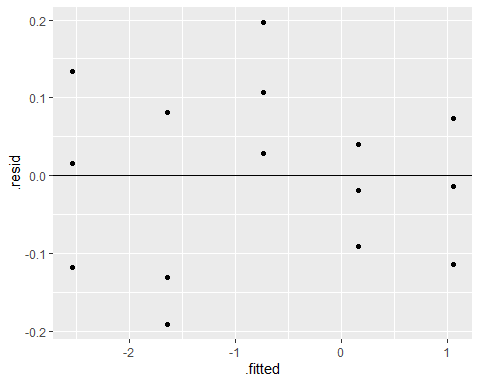
\includegraphics{Homework_4_files/figure-latex/unnamed-chunk-5-1.pdf}

\begin{enumerate}
\def\labelenumi{\arabic{enumi}.}
\tightlist
\item
\end{enumerate}

\begin{Shaded}
\begin{Highlighting}[]
\NormalTok{n }\OtherTok{\textless{}{-}} \FunctionTok{nrow}\NormalTok{(wheat)}
\NormalTok{n}
\end{Highlighting}
\end{Shaded}

\begin{verbatim}
## [1] 21
\end{verbatim}

\begin{Shaded}
\begin{Highlighting}[]
\FunctionTok{tidy}\NormalTok{(lmout, }\AttributeTok{conf.int =} \ConstantTok{TRUE}\NormalTok{)}
\end{Highlighting}
\end{Shaded}

\begin{verbatim}
## # A tibble: 2 x 7
##   term        estimate std.error statistic p.value conf.low conf.high
##   <chr>          <dbl>     <dbl>     <dbl>   <dbl>    <dbl>     <dbl>
## 1 (Intercept)     3.91      1.11      3.52 0.00230     1.58      6.24
## 2 Tcell          10.2       3.30      3.08 0.00611     3.27     17.1
\end{verbatim}

Form the above information, we have a positive linear association
between Tcell and Mass. \texttt{3.91} is the y-intercept of the
regression line. Birds with \texttt{1mm} higher Tcell are estimated to
carry on average \texttt{10.2g} higher stone mass (95\% confidence
interval of \texttt{3.3g} lower to \texttt{17.1g} higher). With a strong
evidence that this association is not due to chance alone \emph{(p =
0.006, n = 21)}.

\begin{enumerate}
\def\labelenumi{\arabic{enumi}.}
\setcounter{enumi}{1}
\tightlist
\item
\end{enumerate}

\begin{Shaded}
\begin{Highlighting}[]
\NormalTok{newbird }\OtherTok{\textless{}{-}} \FunctionTok{data.frame}\NormalTok{(}\AttributeTok{Tcell =} \FunctionTok{c}\NormalTok{(}\FloatTok{0.35}\NormalTok{))}
\FunctionTok{predict}\NormalTok{(}\AttributeTok{object =}\NormalTok{ lmout, }\AttributeTok{newdata =}\NormalTok{ newbird, }\AttributeTok{interval =} \StringTok{"confidence"}\NormalTok{) }\SpecialCharTok{\%\textgreater{}\%} \FunctionTok{cbind}\NormalTok{(newbird)}
\end{Highlighting}
\end{Shaded}

\begin{verbatim}
##        fit      lwr      upr Tcell
## 1 7.469063 6.793505 8.144621  0.35
\end{verbatim}

We estimate that a bird with Tcell of 0.35mm can carry on average a
stone with mass \texttt{7.5g} (95\% confidence interval of 6.8g lower to
8.1g higher).

\begin{enumerate}
\def\labelenumi{\arabic{enumi}.}
\setcounter{enumi}{2}
\tightlist
\item
\end{enumerate}

\begin{Shaded}
\begin{Highlighting}[]
\NormalTok{newbird }\OtherTok{\textless{}{-}} \FunctionTok{data.frame}\NormalTok{(}\AttributeTok{Tcell =} \FunctionTok{c}\NormalTok{(}\FloatTok{0.2}\NormalTok{))}
\FunctionTok{predict}\NormalTok{(}\AttributeTok{object =}\NormalTok{ lmout, }\AttributeTok{newdata =}\NormalTok{ newbird, }\AttributeTok{interval =} \StringTok{"confidence"}\NormalTok{)}
\end{Highlighting}
\end{Shaded}

\begin{verbatim}
##        fit      lwr     upr
## 1 5.944295 4.869499 7.01909
\end{verbatim}

Birds with 0.2mm Tcell are estimated to carry on average \texttt{5.9g}
mass of stone (95\% confidence interval of 4.9g lower to 7.0g higher
mass).

\begin{enumerate}
\def\labelenumi{\arabic{enumi}.}
\setcounter{enumi}{3}
\tightlist
\item
\end{enumerate}

\begin{Shaded}
\begin{Highlighting}[]
\NormalTok{advbird }\OtherTok{\textless{}{-}} \FunctionTok{data.frame}\NormalTok{(}\AttributeTok{Tcell =} \FunctionTok{c}\NormalTok{(}\DecValTok{20}\NormalTok{))}
\FunctionTok{predict}\NormalTok{(}\AttributeTok{object =}\NormalTok{ lmout, }\AttributeTok{newdata =}\NormalTok{ advbird, }\AttributeTok{interval =} \StringTok{"predict"}\NormalTok{)}
\end{Highlighting}
\end{Shaded}

\begin{verbatim}
##        fit      lwr      upr
## 1 207.2137 71.45158 342.9758
\end{verbatim}

We estimate that a "super" bird with Tcell of 20mm can carry on average
\texttt{207.2g} (95\% prediction interval of 71.5g lower to 342.9g
higher).

\end{document}
